\chapter{Stand van zaken}
\label{ch:stand-van-zaken}
\section{Spraakgestuurde technologie}
\label{s:spraakgestuurde technologie}
Er zijn enkele begrippen die met het thema te maken hebben, maar die niet hetzelfde omvatten. Taal- en spraaktechnologie is een verzamelnaam voor allerlei technieken waarmee de computer communiceert met zijn gebruiker door menselijke taal.\autocite{Taalunie2017} Het is de poging van de computer om de menselijke taal na te bootsen.

\subsection{Spraakherkenning}
Spraaktechnologie wordt vaak geassocieerd met spraakherkenning. Volgens \autocite{Rouse2016} is spraakherkenning de kunst van de computer om gesproken taal te identificeren en om te zetten naar voor de computer leesbare machinetaal.
Voor een computer succesvol spraak heeft omgevormd naar tekst, wordt er een lang en moeilijk proces doorlopen. Er wordt kort besproken wat de belangrijkste stappen zijn in het converteren van uitgesproken tekst naar tekst op een computerscherm.
\autocite{Vervoort2017}, \autocite{Geitgey2016} en \autocite{Woodford 2019} beschrijven hoe spraakherkenning in zijn werk gaat.
Wanneer een persoon iets uitspreekt, wordt zijn stem als geluidsgolven opgenomen door een microfoon. De analoge signalen worden omgezet naar digitale door een techniek genaamd sampling. Op vaste intervallen wordt de amplitude van de geluidsgolf gemeten en gedigitaliseerd. Het geluid is omgezet naar bits.

Uit het gedigitaliseerd geluid wordt geprobeerd om zo veel mogelijk ruis te filteren. Daarnaast wordt het ook naar een vast volume en een gelijke snelheid gebracht, omdat niet iedereen even snel en even luid spreekt. De uiteindelijke bedoeling is om een neuraal netwerk in te zetten om klanken en woorden te vormen uit het digitale geluid. Met een neuraal netwerk wordt de techniek bedoeld uit de IT-wereld die de werking van de hersenen gaat nabootsen om een computer zichzelf taken te leren.
Uit deze verkregen verzameling van getallen is het voor een neuraal netwerk nog steeds moeilijk om letters en woorden te herkennen. De bits worden eerst nog gegroepeerd in delen van ongeveer 20 milliseconden lang. Elke groep wordt dan opgesplitst in frequentiebanden waar telkens wordt nagegaan hoeveel energie er in vervat zit. Zo wordt een spectrogram gemaakt die een soort van vingerafdruk voorstelt van het geluid. In deze soort data kan een neuraal netwerk gemakkelijker patronen herkennen.
\begin{figure}[h]
    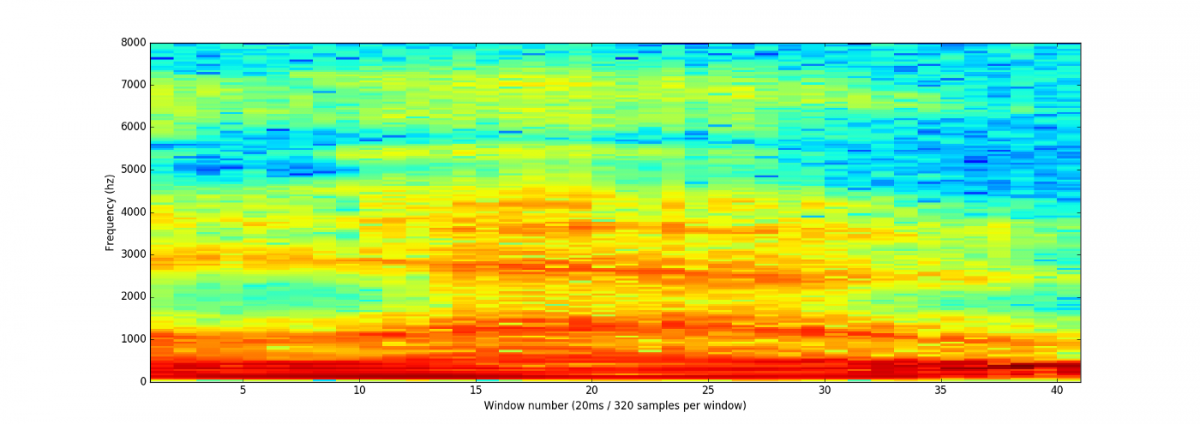
\includegraphics[width=0.7\linewidth]{img/spectogram}
    \caption{een voorbeeld van een spectrogram \autocite{Vervoort2017}}
    \label{fig:spectrogram}
\end{figure}
Dit is het moment waar het neurale netwerk zijn werk begint te doen. Hij gaat aan elk stukje data een spraakklank toekennen. Spraakklanken zijn de klanken die samen een taal vormt. Voor de Nederlandse taal bestaan er 40 verschillende spraakklanken. Klanken worden in woordenboeken fonetisch beschreven om duidelijk te maken hoe woorden worden uitgesproken. Het neurale netwerk gaat uit een fonetische lijst de spraakklank halen die de grootste waarschijnlijkheid heeft om correct bij een audiosignaal te horen. Je kunt nooit helemaal zeker zijn dat er een bepaalde klank is uitgesproken. Dit klinkt eenvoudiger dan het is. Elke klank wordt namelijk door elke mens op een andere manier uitgesproken. Door het netwerk te trainen met een grote hoeveelheid data, zal het beter leren omgaan met deze verscheidenheid.

De laatste stap is het omzetten van de klanken naar woorden. De klanken worden aan elkaar gelinkt tot woorden. Ook hierbij helpt trainingsdata om accurater woorden en zinnen te vormen. Als het netwerk bijvoorbeeld twijfelt tussen de woorden hallo, aloo en haylow, dan zal het waarschijnlijkheid kiezen voor 'hallo' omdat dit waarschijnlijk vaker voorkomt in de trainingsset. Daarnaast houdt het ook rekening met de waarschijnlijkheid dat een bepaald woord volgt op een woord. Ter illustratie, een netwerk zal door te trainen begrijpen dat de kans groter is dat het woord 'voorbeeld' gevolgd is op woorden zoals 'als, een of goed' dan op woorden zoals 'inktvis of tafel'. Voor neurale netwerken populair werden werd hiervoor een andere techniek gebruikt, namelijk het Hidden Markov Model. Hoe dit model precies werkt is buiten de scope van dit onderzoek.

\subsection{Spraaksynthese}
Een andere techniek, die net het omgekeerde is van spraakherkenning, is spraaksynthese. Volgens \autocite{Rouse2016} is spraaksynthese menselijke spraak dat is gevormd door een computer. Spraaksynthese is de basis voor elk Text-To-Speech systeem. Het wordt gebruikt om geschreven tekst om te zetten naar gesproken taal, geproduceerd door de computer.
Spraaksynthese is aanwezig in ons dagelijkse leven. In automatische telefoongesprekken, de luchthaven, gps-systemen, op de bus en natuurlijk in digitale assistenten. \autocite{Seijas2018} vertelt dat er twee soorten van methodes zijn voor Text-To-Speech. Concatenative TTS, waar korte audiofragmenten aaneengeschakeld worden, is daar één van. Het is goed verstaanbaar omdat de woorden zijn opgenomen in hoge kwaliteit, maar het klinkt niet natuurlijk. De andere methode, parametric TTS is een meer statistische methode en  bedenkt de spraak gebaseerd op enkele parameters. Het haalt taalkundige kenmerken uit de tekst. Daarnaast extraheert het vocoder kenmerken die het corresponderende spraaksignaal representeert. Hier wordt niet verder op ingegaan omdat er nu een derde methode is opgedoken.

Deep Learning heeft ervoor gezorgd dat de Text-To-Speechsoftware geavanceerder werd. Eenvoudigweg is deep learning een benaming voor complexe neurale netwerken. 

--Hier nog uitleg over deep learning TTS--
--Hier nog uitleg over spraakhsynthese--
--uitleg over dat neurale netwerken ervoor gezorgd hebben dat deze twee functionaliteiten de drempel haalde van correctheid dat het mogelijk werd om op een aangename en natuurlijke manier met assistenten te communiceren--

Spraaktechnologie omvat naast deze twee begrippen nog meer. Denk maar aan spelling- en grammaticacontrole, spraak- en tekstanalyse, automatische vertalingen, enzovoort.

Spraakherkenning en spraaksynthese zijn nodig in het ontwikkelen van een Voice User Interface (VUI), of stemgestuurde gebruikersomgeving, waar de gebruiker de computer als het ware bedient met zijn stem in plaats van bijvoorbeeld een toetsenbord of aanrakingen. De computer moet gesproken taal van de gebruiker begrijpen (spraakherkenning) en moet een gepast antwoord teruggeven (spraaksynthese). Spraakassistenten zoals Alexa, Siri of Google Assistant zijn voorbeelden van VUI's.

Omdat een assistent de spraak kan omzetten naar tekst betekent dit nog niet dat hij begrijpt wat iemand heeft verteld. Assistenten worden ontwikkeld met Natural Language Processing. Het is een methode om ongestructureerde data gebaseerd op de natuurlijke taal te verwerken tot een vorm die de computer kan begrijpen. Het zorgt ervoor dat de betekenis of het doel wordt achterhaald van wat iemand zegt. NLP valt onder de noemer van Artificiële Intelligentie en het maakt gebruik van deep learning modellen. Modellen die getraind zijn om patronen te gaan herkennen in de menselijke taal door grote hoeveelheden aan data van bijvoorbeeld conversaties en berichten door te nemen. In principe is het vergelijkbaar met hoe een kind de taal leert, namelijk door naar voorbeelden te luisteren. \autocite{Rouse2017}
Volgens \autocite{Garbade2018} kan NLP voornamelijk onderverdeeld worden in twee niveaus, syntaxis en semantiek. Syntaxis is de grammatica van de tekst leren begrijpen. Het splitsen van zinnen of woorden en elk deel identificeren is één van de vele functies. Semantiek is de betekenis van de tekst leren begrijpen. Algoritmen worden gebruikt om bijvoorbeeld woorden te interpreteren en te classificeren als persoonsnaam of plaatsnaam.

\section{Spraakassistenten}
Een spraakassistent, ook wel een virtuele, persoonlijke of slimme assistent genoemd, voert taken uit via verbale instructies van een gebruiker. Het is vooral aanwezig in smartphones, maar het wordt ook geïntegreerd in smart speakers, auto's of wearables. Dit onderzoek vergelijkt twee van de meest prestigieuze assistenten, Google’s Assistant en Amazon’s Alexa. Daarnaast zijn ook Apple's Siri, Microsoft's Cortana en Samsung's Bixby bekende voorbeelden.

\subsection{De geschiedenis van spraakassistenten}
De slimme spraakassistenten zijn vandaag gekend bij het grote publiek. Ze zijn ingebouwd in onze smartphones en slimme luidsprekers. Steeds paraat om ons de vertragingen te melden op de weg, het weer te voorspellen voor morgen of onze favoriete muziek te spelen. Het is iets van deze tijd, maar toch hebben ze al een lang pad van tientallen jaren bewandeld. Dit is hoe het allemaal begon en hoe we zijn geëvolueerd naar de bekende assistenten van vandaag.

\subsubsection{Jaren 50 - 60}
De eerste systemen die ietwat leken op een spraakassistent waren gefocust op het louter herkennen van de menselijke spraak. In \autocite{Vox-Creative2019} wordt geschreven hoe in  de Bell Laboratories in 1952 het ``Audrey'' systeem werd ontwikkeld. Audrey begreep de getallen 0 tot 9 op voorwaarde dat de sprekers tussen elk getal een pauze lieten. In theorie kon het gebruikt worden om met de stem een telefoonnummer in te geven. Onder andere de kost en omvang van de machine was groot. Het intoetsen van de telefoonknoppen bleef efficiënter, dus het effectieve gebruik van Audrey bleef uit.

\autocite{IBM2011} onthulde in 1962 de ``Shoebox'', een machine die met spraakcommando's eenvoudige berekeningen kon uitvoeren. De uitvinder William C. Dersch demonstreerde voor televisie hoe het apparaat, zo groot als een schoendoos, naast de getallen 0 tot 9 ook zes woorden zoals plus en totaal kon herkennen.

\begin{figure}[h]
    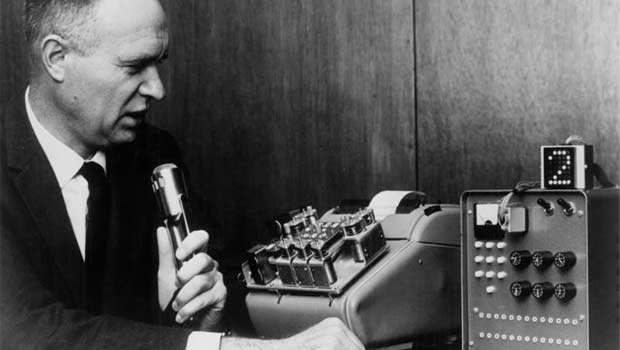
\includegraphics[width=0.7\linewidth]{img/Shoebox}
    \caption{William C. Dersch’s Shoebox deed eenvoudige berekeningen met spraakcommando's \autocite{IBM2011}}
    \label{fig:shoebox}
\end{figure}

\subsubsection{Jaren 70 - 80}
Spraakherkenning in de jaren 70 werd vooral gekenmerkt door het departement voor defensie in de Verenigde Staten. Uit interesse voor spraakherkenning financierden ze een vijfjarig project over het thema. Volgens \autocite{Pinola2011} en \autocite{Kincaid2018} heeft dit geleid tot de ontwikkeling van Harpy in 1976. Harpy begreep 1011 woorden en kreeg vooral betekenis door haar efficiëntere zoekmethode, de ``Beam-search'', om logische zinnen te gaan herkennen.

In \autocite{Pinola2011} staat dat in de jaren 80 er een grote doorbraak kwam door de ontwikkeling van het hidden Markov model. Dit model gebruikt statistieken om een woord te herkennen in een onbekend geluid. Dit werd gedaan door het berekenen van de waarschijnlijkheid dat het onbekend geluid staat voor een bepaald woord. De woordenschat van de spraakherkenningssoftware bleef groeien tot een paar duizend woorden en had dankzij onder andere het hidden Markov model het potentieel om ongelimiteerd woorden te gaan herkennen.
Onder andere dankzij deze ontwikkelingen bleven ook de commerciële toepassingen niet uit. In 1987 kwam de Worlds of Wonder's doll Julie uit. Kinderen konden de pop trainen om te reageren op hun uitspraken. Dit staat zo beschreven in \autocite{Pinola2011}, waar je ook een reclamespot voor de pop kan bekijken. De technologie groeide snel, maar had wel een grote zwakte. De zin moest gedicteerd worden. Na elk woord werd dus een korte pauze verwacht.

\subsubsection{Jaren 90}
Volgens \autocite{Kincaid2018} kwam in de 90's automatische spraakherkenning in een eerste vorm zoals we het vandaag kennen. De doorbraak in die tijd heette Dragon. De eerste versie werd gelanceerd in 1990 onder de naam Dragon Dictate en had een woordenschat van 80 000 woorden. Daarnaast kon het iets nieuws, iets wat in de huidige spraakassistenten nog steeds gebruikt wordt, natural language processing. Zinnen moesten niet meer gedicteerd worden, maar Dragon kon oorspronkelijk 30 tot 40 woorden per minuut herkennen.

Volgens een artikel uit 1998 \autocite{Puri1998} is Dragon verantwoordelijk voor een doorbraak in spraakherkenningssoftware. De opvolger van de Dragon Dictate, Dragon NaturallySpeaking laat gebruikers spreken in een microfoon, aangesloten op de computer, en laat de woorden direct verschijnen op het computerscherm. Indien het een fout maakte, kon je het zelf corrigeren en kon de software leren uit zijn fouten. Het was ook de eerste spraakherkenningssoftware die toeliet om op een normale manier te praten.

\subsubsection{Van 2010 tot nu}
In \autocite{IBM2011} is te lezen hoe een mijlpaal werd bereikt door de Watson machine die won in Jeopardy. Watson was zo goed in taalverwerking dat hij 2 kampioenen in Jeopardy heeft verslaan live op televisie. Jeopardy is een Amerikaans spelprogramma waar de kandidaten het antwoord kregen en ze zelf de bijpassende vraag moesten geven. Watson was niet alleen goed in het samenstellen van correcte vragen, maar kon die ook telkens hardop uitspreken.

\begin{figure}[h]
    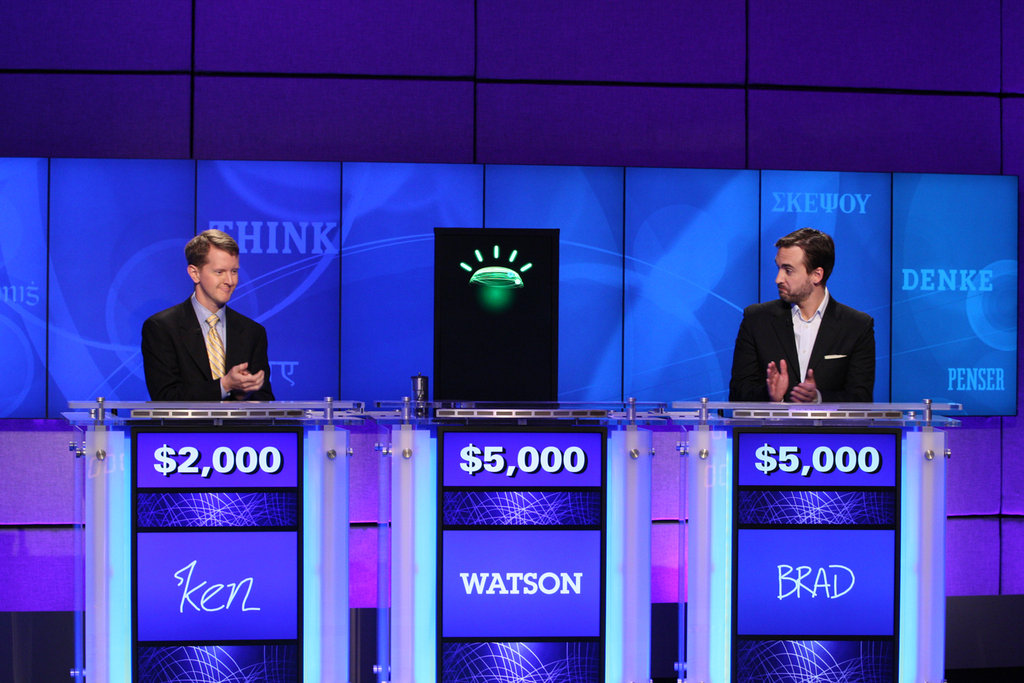
\includegraphics[width=0.7\linewidth]{img/WatsonJeopardy}
    \caption{Watson versloeg twee kampioenen in Jeopardy live op televisie \autocite{Markoff2011}}
    \label{fig:watson}
\end{figure}

\subsection{De spraakassistenten van nu}
--Kostprijs alexa en GA + ondersteuning talen meegeven--
Kort na deze gebeurtenis in 2011 werd Siri gebouwd in de Iphone 4S en werd zo de eerste spraakassistent voor het grote publiek uitgebracht. Siri is Apple's variant op de slimme spraakassistent en is tegenwoordig beschikbaar op meerdere apparaten met een IOS-besturingssysteem. Het grootste aandeel van de gebruikers kent Siri van op zijn Iphone, maar daarnaast is de assistent ook geïntegreerd in de Mac computer, de Apple Watch of de Apple TV. Ondertussen heeft het ook zijn eigen Smart Speaker, de HomePod.

Google gaf hierop een antwoord in 2012 door Google Now uit te brengen, de voorloper van de Google Assistant van vandaag. Volgens Google is de Google Assistant jouw eigen persoonlijke Google, die altijd bereid is om je te helpen wanneer je maar wilt. De Google Assistant bestond eerst onder de naam Google Now en was aanwezig in smartphones met een Android besturingssysteem. De Google Assistant van vandaag is te vinden in veel meer omgevingen. Smartphones, auto's, laptops, tablets, tv's, smartwatches en in hun eigen smart speaker, de Google Home. Deze speaker heeft ook een variant gekregen met een scherm, de Smart Display.

Tijdens de Microsoft BUILD conferentie in 2013 werd Cortana geïntroduceerd als de spraakassistent van Microsoft. Cortana is ontwikkeld voor onder andere Windows 10, Windows Phone, Xbox One en in de slimme speaker Invoke.

In 2015 kwam de eerste slimme luidspreker op de markt. De Echo van Amazon, voorzien met hun slimme spraakassistent, Alexa. Amazon is één van 's werelds grootste bedrijven in het online verkopen van goederen. Het grote verschil met Google is dat de assistent voor het eerst werd gebruikt in de Echo, Amazon's smart speaker. Een groot nadeel aan Alexa is dat het vooral focust op de Amerikaanse markt en dus ook geen Nederlands kan.

\autocite{Lopez2018} besprak verschillende functionaliteiten van spraakassistenten Google Assistant, Alexa en Siri, op correctheid en natuurlijkheid bij 8 ondervraagden. In de administratieve categorie, zoals agendabeheer, to-dolijsten en alarmen kwam de Google Assistant als minst correct en minst natuurlijke assistent uit de bus, maar prijkt in de veelzijdige categorie (nieuws, weer, verkeer, woordbetekenissen, rekenen,, enz.) dan weer ver bovenaan op beide vlakken. Algemeen werd de Google Assistant als de meest natuurlijke ervaren, onder andere door de toon van de stem die verwondering, onzekerheid en vreugde uitte.
Voor \autocite{Tulshan2019} stelden 100 personen allerlei vragen aan voice assistants Google Assistant, Alexa, Siri en Cortana. Ze gaven telkens een score op spraakherkenning en contextueel inzicht. Google Assistant kwam als grote winnaar uit het onderzoek door 59,80 \% van de vragen te beantwoorden. Een verschil van 15,82 \% met Siri, die de op één na nauwkeurigste bleek in dit onderzoek. Google Assistant was vooral leider in categoriëen als reizen, mailing, navigatie, vertalingen en begreep volgens het onderzoek goed de verschillende variaties in de stemmen van de onderzochte personen.

Volgens \autocite{Lopez2018} is de Echo Dot de favoriete smart speaker als het aankomt op het aankopen van artikelen. Dit is geen verrassing omdat hij oorspronkelijk ontworpen is om te winkelen en zelfs de enige spraakassistent is waarmee je online kan shoppen. In \autocite{Tulshan2019} bleek Alexa de minst nauwkeurige assistent te zijn met 7,91 \% nauwkeurigheid.

Google spendeert veel middelen aan zijn assistent. Het heeft indruk gemaakt tijdens de recente Google I/O conferentie van dinsdag 7 mei 2019, waar ze onverwachts nieuws brachten. De volgende versie van de Google Assistant zal namelijk opvallend veel sneller gaan omdat ze de AI-modellen die verantwoordelijk zijn voor NLP offline beschikbaar hebben gemaakt. Dat wilt zeggen dat een commando van een gebruiker niet meer helemaal naar een server in Amerika moet transporteren om ervoor te zorgen dat de assistent het kan begrijpen. Vanaf de volgende versie zal deze logica afgehandeld worden door uw toestel zelf, omdat Google erin geslaagd is het geheugen van die modellen zo te reduceren dat het kan opgeslagen worden op uw apparaat. Het belooft dus dat binnenkort de gebruiker na het stellen van een vraag amper nog zal moeten wachten op een antwoord.

VRT NWS meldt op 28 mei dat de Belgische variant van de Google Assistant wordt gelanceerd. \autocite{Belghmidi2019} Voorlopig nog alleen met een Nederlands accent. Wat er wel bijkomt is de samenwerking met verschillende Belgische bedrijven. Zo kan iedereen binnenkort via de Google Assistant naar het radionieuws van VRT NWS luisteren, aan de NMBS vragen wanneer de volgende trein komt of artikelen van de Colruyt toevoegen aan zijn lijstje.

Slimme spraakassistenten worden alleen maar slimmer. \autocite{Brandt2018} heeft onderzocht hoe hoog het intelligentieniveau is van 4 slimme assistenten, namelijk Google Assistant, Microsoft Cortana, Amazon Alexa en Apple Siri in 2017 en 2018. De geanalyseerde gegevens zijn de antwoorden van de assistenten op 5000 algemene vragen. De beste prestatie werd verricht door Google Assistant die op 77,2 procent van de vragen een antwoord kon bieden, waarvan 95 procent correct. Bij alle assistenten zie je een verhoging van de intelligentie in vergelijking met het vorige jaar.

\begin{figure}[h]
    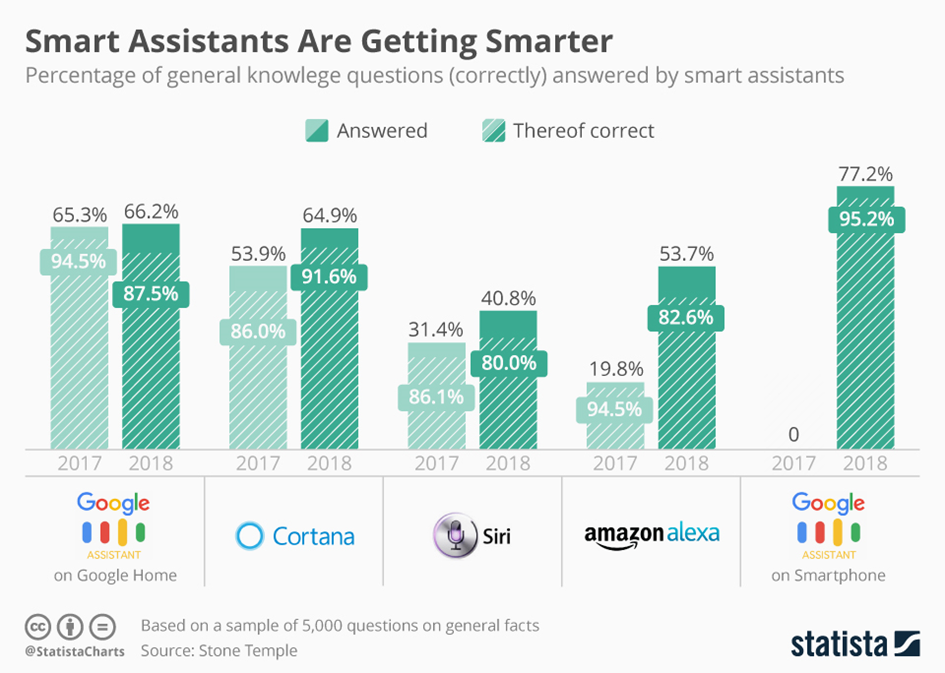
\includegraphics[width=0.7\linewidth]{img/SmartAssistantsAreGettingSmarter}
    \caption{Hoe hoog ligt het intelligentieniveau bij slimme spraakassistenten \autocite{Brandt2018}}
    \label{fig:smartassistantsaregettingsmarter}
\end{figure}

--Hier nog verder doen met overige bronnen over assistenten vandaag--

Als het gaat over de spraakkwaliteit, ook meer uitleggen wat er precies is beoordeeld.
-> De Text-to-speech of speech synthesis, bij Google Assistant met WaveNet: https://towardsdatascience.com/wavenet-google-assistants-voice-synthesizer-a168e9af13b1

\subsection{Hoe werkt een spraakassistent}
--De flow uitleggen van de gebruiker die iets vraagt tot de assistent die een antwoord heeft gegeven--

\section{Bestaande eerste hulpapplicaties}
\subsection{De Vlaamse EHBO-app van het Rode Kruis}
Op 2 april ’19 kwam het Rode Kruis met het nieuws dat ze een app hebben ontwikkeld die kan helpen bij het geven van eerste hulp bij ongevallen. 80 procent van de Vlamingen weet niet wat hij moet doen als een nabije persoon begint te stikken, een hartstilstand krijgt of hevig begint te bloeden. Uit angst om iets fouts te doen, gebeurt er dan ook vaak niks. Met de app willen ze zoveel mogelijk mensen in staat stellen om hulp te verlenen. \autocite{Decroubele2019}

Het Rode Kruis benadrukt dat de applicatie de opleiding niet kan vervangen, maar dat het hulp kan bieden bij het geven van eerste hulp.

In de applicatie zijn er drie grote onderdelen, eerste hulp verlenen, eerste hulp leren en een AED-toestel vinden in de buurt. Er zijn ook nog enkele opties die je naar de website van het Rode Kruis brengen om informatie te verkrijgen over het geven van bloed of plasma, het doen van een gift, het volgen van een opleiding of het aanmelden als vrijwilliger.

Als je eerste hulp wilt verlenen kun je uit het overzicht een onderwerp over eerste hulp kiezen, waarna je informatie krijgt over wat je moet vaststellen en wat je nodig hebt. Daarnaast geeft de app ook een stappenplan van instructies wat je moet doen. De levensbedreigende situaties staan helemaal bovenaan en zijn voorzien van extra ingesproken instructies.

Als je eerste hulp wilt leren kun je eerst een onderwerp kiezen. Voorbeelden zijn een beroerte of alcoholvergiftiging. Daarna krijg je over het onderwerp vragen \& antwoorden, informatieteksten en video's. Per leerdeel krijg je een quiz die je moet oplossen om bepaalde badges te verdienen.

Wanneer iemand in uw omgeving een hartstilstand krijgt dan kun je met de applicatie een kaart openen waar AED-toestellen staan op gesitueerd. Je kunt er ook een nieuwe AED melden of meer informatie lezen.


\subsection{Andere EHBO-applicaties}
Nederland heeft al langer een mobiele EHBO-applicatie. Deze verschilt niet zo veel met de Belgische versie. Ze heeft wel een zoekfunctie om sneller de instructies voor uw ongeval te vinden. Je kan er ook EHBO-kits en cursussen bestellen in de webshop.

--Nog iets over Engelstalige applicaties--
